\subsection{Computation} 

%\TODO{--CHECK--}
The general idea to compute a kNN, is to (i) calculate the distance between $r_i$ and $s_j$ for all $i$ and all 
$j$, and (ii) sort these distances in ascending order to 
find out the first $k$ results. In MapReduce, the idea is the same except that what is given to a task must be independent in order to ensure correctness without duplicating the whole dataset. The number of MapReduce jobs used for computing and sorting has
an impact on the global performance, given the complexity of the computation performed by each task and the amount of data to exchange between them. 
The preprocessing and partitioning steps can also affect the number of tasks that are further needed by each MapReduce job. 
%Also, the pre-processing and the partitioning of the data can also be performed with MapReduce. Hence, 
%depending on the chosen workflow, many different jobs are involved. 
In this section, we review the 
different strategies used to compute and sort distances efficiently using MapReduce. These different strategies can be divided into two categories: the ones 
using one round of MapReduce job and the ones using two rounds of MapReduce jobs. Then, those categories can be divided into two subcategories: the ones that do 
not preprocess and partition data before computation and the ones that implement the preprocessing and partitioning steps. We detail all these 
strategies in the following.

\subsubsection{One Round of MapReduce Job}

\textbf{Without preprocessing and partitioning.} 
The basic idea (H-BkNNJ) to compute a kNN with MapReduce is to have every Map task process a 
pair of $R_i$ and $S_j$, and perform a block nested loop on them to calculate the distance between $r_i \in 
R_i$ and $s_j \in S_j$,  $\forall$ $i$ and $j$. Note that, without any smart partitioning strategy, every possible blocks of one partition $R_i$ from $R$ and $S_j$ from $S$ should be calculated, leading to $n^2$ tasks totally where n is the number of partitions of $R$ and $S$.
%$S_j$ must represent the whole dataset $S$ to produce a correct output.
The output of the Map task is in the form of $\left(id(r_i), list
\left( id(s_{j}), d\left(r_i, s_j\right)\right)\right)$. The identifier of $r_i$, named $id(r_i)$, is used as a key and the 
associated value is a list containing the identifier of $s_j$ and the computed distance between $r_i$ and $s_j$. A reduce task then 
processes all computed distances for a given $r_i$, and sorts them in ascending order to 
output the top $k$ results. 
%This basic idea is explained in more details in \cite{Zhang:2012:EPK:2247596.2247602}.
%tasks will take the same partitions from the output of the Map tasks, merge all the results of the same key 
%together and sort $d\left(r_i, s_j\right)$ 
%in a descending order, and emit the top $k$ results. 
%Figure~\ref{knn_mapreduce} shows the basics of this process.
%\begin{figure}[t]
%\center
%\scalebox{0.3}{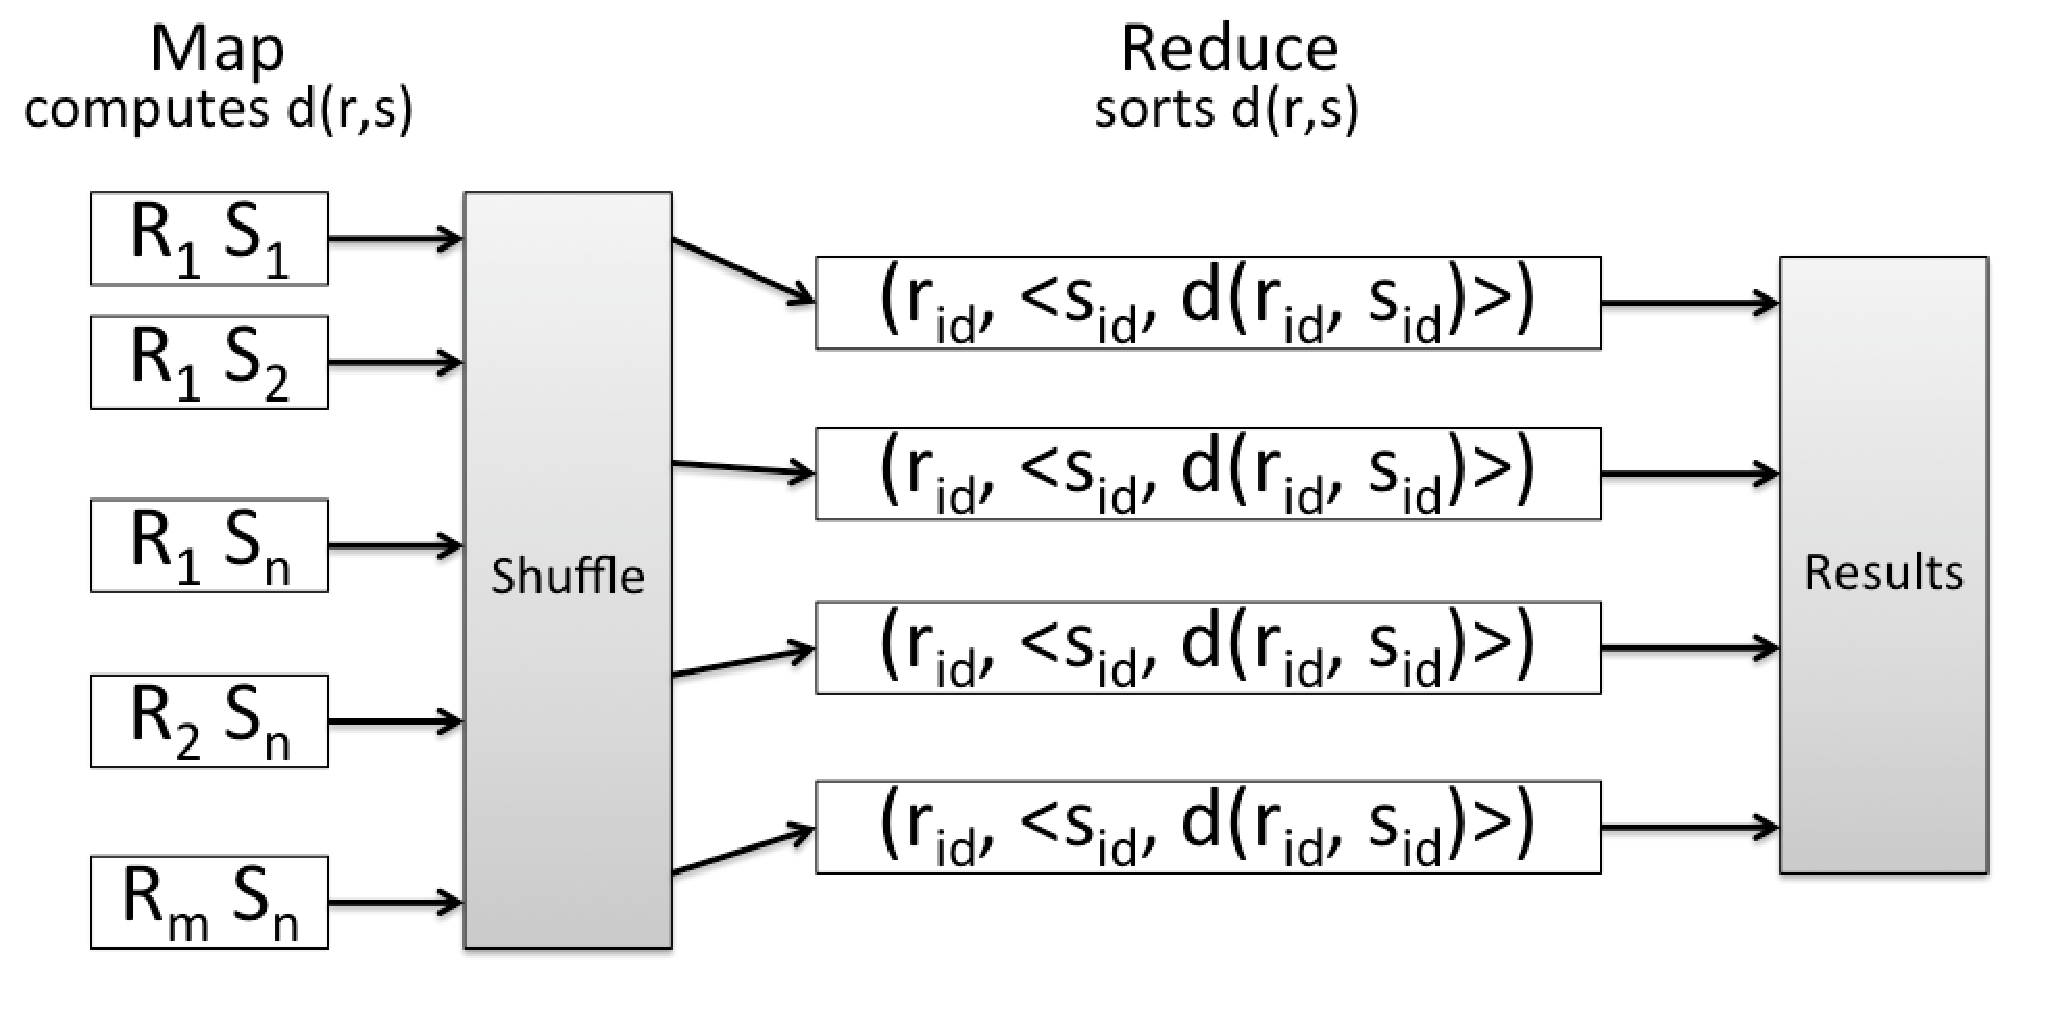
\includegraphics{res/knn-mapreduce.pdf}}
%\caption{Basic idea for processing kNN join in MapReduce \label{knn_mapreduce}}
%\end{figure}
\begin{figure*}[t]
\center
\scalebox{0.35}{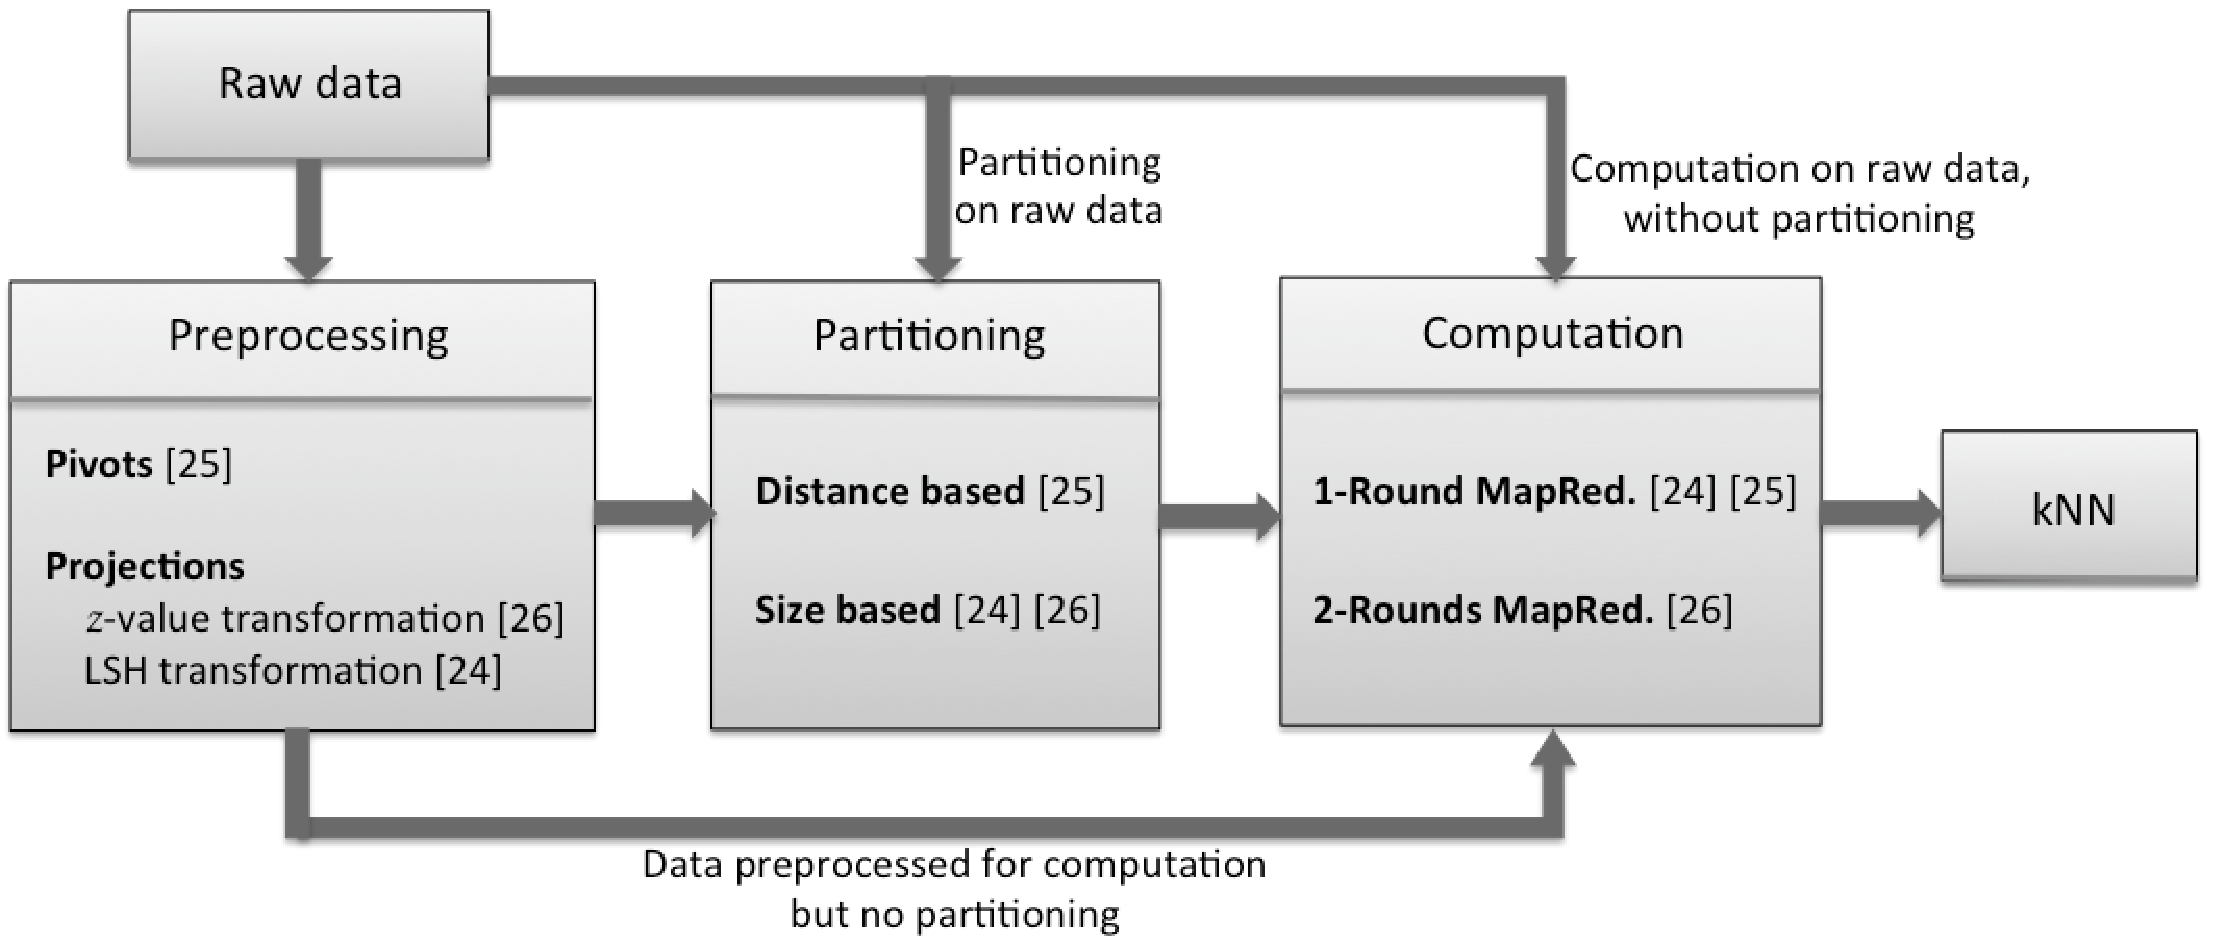
\includegraphics{res/workflow.pdf}}
\caption{Usual workflow of a kNN computation using MapReduce \label{workflow}}
\end{figure*}


\textbf{With preprocessing and partitioning.} To reduce the number of tasks used to calculate the distances, in other words, to reduce the number of pairs formed by $R_i$ and $S_j$, PGBJ \cite{Lu:2012:EPK:2336664.2336674} uses a preprocessing and distance based partitioning strategy, which ensures that each partition $R_i$ has only one corresponding partition $S_i$ needed to be searched, which reduces the number of tasks to $n$. %In this work, 
%they pre-select similar objects (close points) in $R$ and form a partition with them using distance based partitioning 
%\TODO{not already explained in previous section? --CHECK--}
%, and they subsequently find the 
%corresponding partition in $S$. 
Once the blocks of $R_i$ and $S_i$ identified, they perform the same calculation as in the H-BkNNJ technique. Because of 
their data organization, they are able to reduce the number of tasks, greatly improving the performance.

In RankReduce \cite{Stupar10rankreduce-}\footnote{Although RankReduce only compute kNN for a single query, it is 
easy to extend it to a full kNN join}, the authors first preprocess and partition data into buckets using 
LSH. Their Map function computes the distance of all points in the partition, and then sorts the local distances to output the local 
 $k$ nearest neighbors for each point in the partition, together with their distance in form of $\left(id(r_i), list
\left( id(s_{j}), d\left(r_i, s_j\right)\right)\right)$.
 %$\left(query, \left(neighbor, distance\right)\right)$. 
 %\TODO{why don't we have the same notation than before with ri, d() ...}
These key-value pairs are then pulled by Reducers where they are sorted and issued as final results.

Overall, the main limitation of these approaches is that the number of values to be sorted in the reduce phase
can be extremely large, up to $\left|S\right|$, if the
pre-processing and partitioning have not significantly reduced the set of candidate points.
%when the filtering on the reference points is too coarse. \TODO{reference points? can we say: if the
%pre-processing and partitioning have not significantly reduced the set of candidates}.
%\TODO{I don't like partitioning here, another word like filtering? -- ?? --}. 
This greatly limits the applicability of such approach. 


\subsubsection{Two Rounds of MapReduce Jobs}
\textbf{Without preprocessing and partitioning.} 
To overcome the previously described limitation, multiple successive MapReduce jobs are required. The idea is to have the first job output
the top $k$ for each pair ($R_i$, $S_j$). Then, the second job is used to merge all the top $k$ values for a 
given $r_i$ and to perform the merging and sorting of all local top $k$ values (instead of all values), producing the final global top $k$. Such approach is used in H-BNLJ 
\cite{Zhang:2012:EPK:2247596.2247602} and greatly improves sorting time. %And the authors also indicate that we can index the local blocks of S by R-Tree and improve H-BNLJ to H-BRJ.\TODO{is this related to this section?}

%H-BkNNJ method only uses one MapReduce job, but we need to sort $\left|S\right|$ numbers of $d\left(r_i, s_j\right)$ for every object $r_i$. The sort
%algorithm in MapReduce is Quick Sort and Merge Sort by default, their complexity is $\left|S\right| \times Log \left|S\right|$. When $\left|S\right|$ is 
%large, this process is very time consuming. So, paper \cite{Zhang:2012:EPK:2247596.2247602} gives an improvement H-BNLJ. H-BNLJ uses two MapReduce jobs 
%to achieve the same goal. Mapper 1 will get a piece of $R_i$ and $S_j$, Reducer 1 will calculate the distance between $\forall$ $r_i \in R_i$ and $s_j 
%\in S_j$, Mapper 2 sort the results of Reducer 1 and emit the local top $k$ results, Reducer 2 pull the local result of the same key, merge and sort them 
%then give the global top $k$ results. The authors also point out that we can use some index structures like R-Tree to index the local $S$ blocks in order 
%to speed up finding the nearest neighbors.


\textbf{With preprocessing and partitioning.} 
A last possibility is based on the z-value preprocessing.
%the two previous methods: one job for pre-processing and partitioning, one for 
%computing the distances, and a lost one for filtering and sorting the results. 
In H-zkNNJ \cite{Zhang:2012:EPK:2247596.2247602} the authors propose to generate several shifted copies of $R$ and $S$ (to improve the 
accuracy), and to determine the bounds of the partitions of $R_i$ and the 
corresponding $S_i$ in a pre-processing MapReduce job. So here, the preprocessing and partitioning step is completely integrated in MapReduce. Then, the first MapReduce round of computation takes the partitions $R_i$ and $S_i$ previously determined, and computes the candidate neighbor set, named 
$C_i\left(r\right)$,  for $\forall r_i \in R_i$, which contains $k$ local nearest objects immediately before $r_i$ and $k$ objects after $r_i$ ($2k$ objects totally). %\TODO{not clear. Notation seems inconsistent, why r and not r\_i?}
The second MapReduce round decides the exact result $\forall r_i \in R$ from the candidate neighbor set $kNN\left(r, C_i\left(r\right)\right)$.
%\TODO{how? what does the job do in practice?}
%\TODO{don't like kNN(r,...) here, can it be simpler?}
So in total, three MapReduce jobs are launched, and among them, two are actually devoted to the kNN computation. As the number of points that are in the candidate neighbor set is small, thanks to the drastic partitioning (itself due to a drastic preprocessing), the cost of computation and communication is extremely reduced.
